The backend uses the dotNet framework.
In the dotNet framework, development is done using the C\# language. 
The Onion Architecture is adopted,
The Onion Architecture is a typical layered architecture, 
where each layer depends on the inner layer and provides interfaces to the outer layer.
The outer layer provides services to the outermost layer 
and other modules in the same layer based on the interfaces of the inner layer.

From inner to outer, the layers are: Domain, Application, Infrastructure, Presentation.
The Domain layer is the core layer and the innermost layer, used to define domain models, 
which are the business models.
It includes domain models and domain service interfaces.
Domain models are used to define the business models, 
which are the entities in the entity-relationship model and their attributes.
Domain service interfaces are used to define the business services, 
which are the relationships between entities in the entity-relationship model.

The Application layer is the application layer, 
used to define application services, which are the business logic.
It includes domain service implementations and application service interfaces.
Domain service implementations implement the methods of the inner layer's domain service 
interfaces and implement the business logic of the domain models.
Application service interfaces are used to define application services, 
which are the business logic.
It includes but is not limited to database interfaces, testing interfaces, 
HTTP API interfaces, MQTT interfaces, etc.

The Infrastructure layer is the infrastructure layer, used to define infrastructure.
It includes database implementations, testing implementations, 
HTTP API implementations, MQTT implementations, etc.
Database implementations implement the database interfaces 
and provide CRUD services for the database.
Testing implementations implement the testing interfaces 
and provide services for unit testing and integration testing.
HTTP API implementations implement the HTTP API interfaces 
and provide CRUD operations for HTTP APIs.
MQTT implementations implement the MQTT interfaces 
and provide CRUD operations for MQTT.

The Presentation layer is the presentation layer, used to define presentation logic, 
such as interfaces and pages. Since this is a backend project,
data presentation and control are handled by the frontend, 
so this layer is not needed.


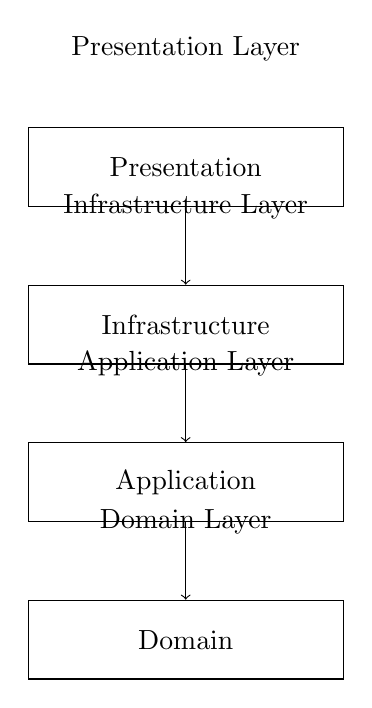
\begin{tikzpicture}[node distance=2cm, every edge/.style={draw, thick}]
    % Layers
    \node[rectangle, draw, minimum width=4cm, minimum height=1cm] (presentation) {Presentation};
    \node[rectangle, draw, minimum width=4cm, minimum height=1cm, below of=presentation] (infrastructure) {Infrastructure};
    \node[rectangle, draw, minimum width=4cm, minimum height=1cm, below of=infrastructure] (application) {Application};
    \node[rectangle, draw, minimum width=4cm, minimum height=1cm, below of=application] (domain) {Domain};

    % Dependencies
    \draw[->] (presentation) -- (infrastructure);
    \draw[->] (infrastructure) -- (application);
    \draw[->] (application) -- (domain);

    % Labels
    \node[above of=presentation, yshift=-0.5cm] {Presentation Layer};
    \node[above of=infrastructure, yshift=-0.5cm] {Infrastructure Layer};
    \node[above of=application, yshift=-0.5cm] {Application Layer};
    \node[above of=domain, yshift=-0.5cm] {Domain Layer};
\end{tikzpicture}

